\begin{event}{AMRS2018: Conference on Applied Mathematics and Random Structures}{AMRS2018}{Birzeit, Palestine, 27th-30th of August 2019}
{Paris 13 University}{41}{1}{https://lipn.univ-paris13.fr/~nicodeme/birzeit18RAND/}

\textbf{Main goals.}AMRS is a conference intended to foster collaborations between Palestinian and French universities or research centres; 
to sustain the critical efforts of the mathematics community in Palestine to set up a doctoral school. AMRS provided an opportunity for dissemination of important and recent results in the field of Applied Mathematics and Statistics with Applications to Economy, Industry, and Science.

\textbf{\ODK implication.}
\ODK was coorganizer for the conference and funded the travel costs
for Sage developer Thierry Monteil to deliver a Sage tutorial.

\textbf{Event summary.}
AMRS conference gathered 41 attendees around various fields of Applied mathematics: Statistics, Game Theory, Analytic Combinatorics, 
Probability, Differ-ential or Difference Equations, Matrices,
Stochastic Optimal Control Problems, Partial Differential Equations, 
Binary Search Trees, Ideals on Skew Matrices. 
There were 13 talks given by 7 Palestinian professors, and 6 French); and 10 talks by students:

\textbf{Results and impact.}

Thierry Monteil introduced the basic concepts of Sage and presented
many examples based on graphs algorithms to 24 students: 19 from
Birzeit– 3 from Al Quds– 1 from Polytechnic Palestine University
Hebron (PPU)– 1 from Malaya. 19 of the 24 students were female.


\begin{figure}[ht]
  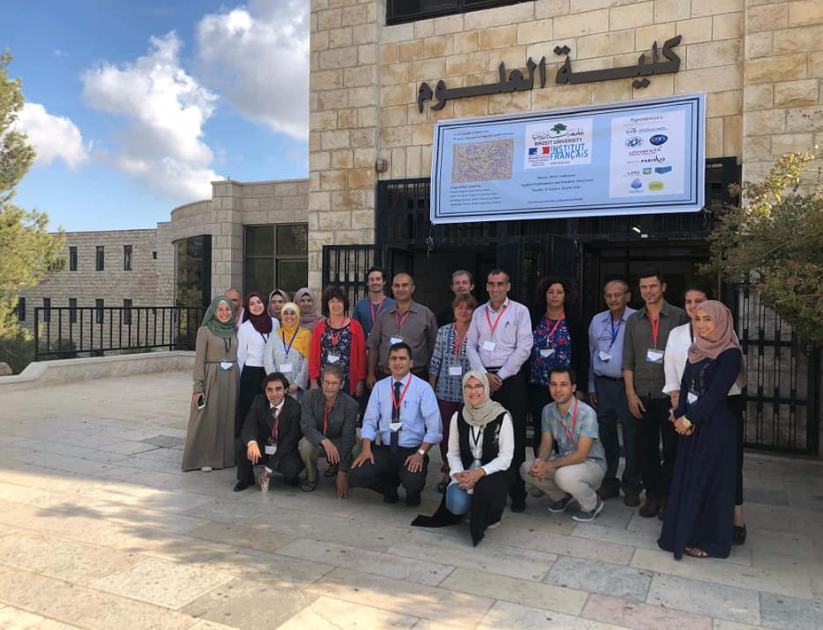
\includegraphics[width=.75\textwidth]{AMRS.png}
  \caption*{AMRS2018}
\end{figure}

\end{event}
